% Copyright © 2012, 2014 Martin Ueding <dev@martin-ueding.de>
%
% Copyright © 2012 Martin Ueding <dev@martin-ueding.de>
%
\documentclass[11pt, ngerman, fleqn]{scrartcl}

\usepackage{graphicx}

%%%%%%%%%%%%%%%%%%%%%%%%%%%%%%%%%%%%%%%%%%%%%%%%%%%%%%%%%%%%%%%%%%%%%%%%%%%%%%%
%                                Locale, date                                 %
%%%%%%%%%%%%%%%%%%%%%%%%%%%%%%%%%%%%%%%%%%%%%%%%%%%%%%%%%%%%%%%%%%%%%%%%%%%%%%%

\usepackage{babel}
\usepackage[iso]{isodate}

%%%%%%%%%%%%%%%%%%%%%%%%%%%%%%%%%%%%%%%%%%%%%%%%%%%%%%%%%%%%%%%%%%%%%%%%%%%%%%%
%                          Margins and other spacing                          %
%%%%%%%%%%%%%%%%%%%%%%%%%%%%%%%%%%%%%%%%%%%%%%%%%%%%%%%%%%%%%%%%%%%%%%%%%%%%%%%

\usepackage[activate]{pdfcprot}
\usepackage[left=3cm, right=2cm, top=2cm, bottom=2cm]{geometry}
\usepackage[parfill]{parskip}
\usepackage{setspace}

\setlength{\columnsep}{2cm}

%%%%%%%%%%%%%%%%%%%%%%%%%%%%%%%%%%%%%%%%%%%%%%%%%%%%%%%%%%%%%%%%%%%%%%%%%%%%%%%
%                                    Color                                    %
%%%%%%%%%%%%%%%%%%%%%%%%%%%%%%%%%%%%%%%%%%%%%%%%%%%%%%%%%%%%%%%%%%%%%%%%%%%%%%%

\usepackage{color}

\definecolor{darkblue}{rgb}{0,0,.5}
\definecolor{darkgreen}{rgb}{0,.5,0}
\definecolor{darkred}{rgb}{.7,0,0}

%%%%%%%%%%%%%%%%%%%%%%%%%%%%%%%%%%%%%%%%%%%%%%%%%%%%%%%%%%%%%%%%%%%%%%%%%%%%%%%
%                         Font and font like settings                         %
%%%%%%%%%%%%%%%%%%%%%%%%%%%%%%%%%%%%%%%%%%%%%%%%%%%%%%%%%%%%%%%%%%%%%%%%%%%%%%%

\usepackage[charter, greekuppercase=italicized]{mathdesign}
\usepackage{beramono}
\usepackage{berasans}

% Style of vectors and tensors.
\newcommand{\tens}[1]{\boldsymbol{\mathsf{#1}}}
\renewcommand{\vec}[1]{\boldsymbol{#1}}

%%%%%%%%%%%%%%%%%%%%%%%%%%%%%%%%%%%%%%%%%%%%%%%%%%%%%%%%%%%%%%%%%%%%%%%%%%%%%%%
%                               Input encoding                                %
%%%%%%%%%%%%%%%%%%%%%%%%%%%%%%%%%%%%%%%%%%%%%%%%%%%%%%%%%%%%%%%%%%%%%%%%%%%%%%%

\usepackage[T1]{fontenc}
\usepackage[utf8]{inputenc}

%%%%%%%%%%%%%%%%%%%%%%%%%%%%%%%%%%%%%%%%%%%%%%%%%%%%%%%%%%%%%%%%%%%%%%%%%%%%%%%
%                         Hyperrefs and PDF metadata                          %
%%%%%%%%%%%%%%%%%%%%%%%%%%%%%%%%%%%%%%%%%%%%%%%%%%%%%%%%%%%%%%%%%%%%%%%%%%%%%%%

\usepackage{hyperref}
\usepackage{lastpage}

\hypersetup{
	breaklinks=false,
	citecolor=darkgreen,
	colorlinks=true,
	linkcolor=black,
	menucolor=black,
	pdfauthor={Martin Ueding},
	urlcolor=darkblue,
}

%%%%%%%%%%%%%%%%%%%%%%%%%%%%%%%%%%%%%%%%%%%%%%%%%%%%%%%%%%%%%%%%%%%%%%%%%%%%%%%
%                               Math Operators                                %
%%%%%%%%%%%%%%%%%%%%%%%%%%%%%%%%%%%%%%%%%%%%%%%%%%%%%%%%%%%%%%%%%%%%%%%%%%%%%%%

\usepackage[thinspace, squaren]{SIunits}
\usepackage{amsmath}
\usepackage{amsthm}
\usepackage{commath}

% Word like operators.
\DeclareMathOperator{\arcsinh}{arsinh}
\DeclareMathOperator{\arsinh}{arsinh}
\DeclareMathOperator{\asinh}{arsinh}
\DeclareMathOperator{\card}{card}
\DeclareMathOperator{\diam}{diam}
\renewcommand{\Im}{\mathop{{}\mathrm{Im}}\nolimits}
\renewcommand{\Re}{\mathop{{}\mathrm{Re}}\nolimits}

% Special single letters.
\DeclareMathOperator{\fourier}{\mathcal{F}}
\newcommand{\C}{\ensuremath{\mathbb C}}
\newcommand{\ee}{\mathrm e}
\newcommand{\ii}{\mathrm i}
\newcommand{\N}{\ensuremath{\mathbb N}}
\newcommand{\R}{\ensuremath{\mathbb R}}

% Shape like operators.
\DeclareMathOperator{\dalambert}{\Box}
\DeclareMathOperator{\laplace}{\bigtriangleup}
\newcommand{\curl}{\vnabla \times}
\newcommand{\divergence}[1]{\inner{\vnabla}{#1}}
\newcommand{\vnabla}{\vec \nabla}

% Shortcuts
\newcommand{\ev}{\hat{\vec e}}
\newcommand{\e}[1]{\cdot 10^{#1}}
\newcommand{\half}{\frac 12}
\newcommand{\inner}[2]{\left\langle #1, #2 \right\rangle}

% Placeholders.
\newcommand{\emesswert}{\del{\messwert \pm \messwert}}
\newcommand{\fehlt}{\textcolor{darkred}{Hier fehlen noch Inhalte.}}
\newcommand{\messwert}{\textcolor{blue}{\square}}
\newcommand{\punkte}{\textcolor{white}{xxxxx}}


\usepackage{float}
\usepackage{scrpage2}
\usepackage{tikz}

\newcommand{\themodul}{physik311}
\newcommand{\thegruppe}{Gruppe 3 -- Matthias Rehberger}
\newcommand{\theuebung}{11}

\pagestyle{scrheadings}

\cfoot{\footnotesize{\thegruppe}}
\ifoot{\footnotesize{Martin Ueding}}
\ofoot{\footnotesize{Seite \thepage\ / \pageref{LastPage}}}
\ihead{\themodul{} -- Übung \theuebung}
\ohead{\rightmark}
\chead{}
\setheadsepline{.4pt}
\automark{section}

\setcounter{section}{36}


\def\thesubsection{\thesection\alph{subsection}}

\title{\themodul{} -- Übung \theuebung \\ \vspace{0.5cm} \large{\thegruppe}}

\author{Martin Ueding \\ \small{\href{mailto:mu@uni-bonn.de}{mu@uni-bonn.de}}}

\begin{document}

\maketitle

\begin{table}[h]
	\centering
	\begin{tabular}{l|c|c|c|c}
		Aufgabe & \ref 1 & \ref 2 & \ref 3 & $\sum$   \\
		\hline
		Punkte & \punkte & \punkte & \punkte & \punkte
	\end{tabular}
\end{table}

%%%%%%%%%%%%%%%%%%%%%%%%%%%%%%%%%%%%%%%%%%%%%%%%%%%%%%%%%%%%%%%%%%%%%%%%%%%%%%%
%                            Fourier-Spektrometer                             %
%%%%%%%%%%%%%%%%%%%%%%%%%%%%%%%%%%%%%%%%%%%%%%%%%%%%%%%%%%%%%%%%%%%%%%%%%%%%%%%

\section{Fourier-Spektrometer}
\label 1

In welche Richtung wird der Spiegel bewegt? Ich nehme an, dass er in
Strahlrichtung bewegt wird.

\subsection{}

Die Intensität hatte ich auf einem vorherigen Aufgabenblatt (Aufgabe 29a)
bestimmt. Dabei war die Intensität als Funktion des Gangunterschieds $\delta$
gegeben durch:
\[
	I(\delta) = 2 I_0 \del{1 + \cos\del\delta}
\]

Die zusätzliche Weglänge $\Delta$, die das Licht zurücklegen muss ist
$\Delta(t) = 2 v t$, dabei habe ich $\Delta(0) = 0$ gewählt. Der
Gangunterschied ist mit der Wellenzahl $k = 2 \pi f / c$:
\[
	\delta(t) = 4 \pi v t \frac fc
\]

Dies setze ich in $I(\delta)$ ein und erhalte:
\[
	I(t) = 2 I_0 \del{1 + \cos\del{4 \pi v \frac fc t}}
\]

\subsection{}

Beim Helium-Neon-Laser überlagern sich die drei Frequenzen. Die
Gangunterschiede $\Delta = 2 vt$ sind für alle Frequenzen gleich. Aufgrund der
unterschiedlichen Wellenzahlen sind die Phasenunterschiede $\delta_i$
allerdings nicht gleich. Außerdem können selbst bei $\Delta = 0$ schon
Phasenunterschiede durch die unterschiedlichen Frequenzen auftreten. Ich nehme
ohne Beschränkung der Allgemeinheit an, dass das Interferometer so bemessen
ist, dass für $\Delta = 0$ alle $\delta_i = 0$ sind.

Der Phasenunterschied der Wellen zur ersten Welle ist:
\[
	\delta_i
	= \underbrace{k_i \Delta}_\text{Gangunterschied}
	+ \underbrace{\del{\omega_1 - \omega_i} t}_\text{Schwebung}
\]

Dabei ist $\omega_1 - \omega_i = \pm 2 \pi a$ für die Wellen $2$ und $3$. Insgesamt interferieren $6$ Wellen miteinander, die folgende Phasenunterschiede bezogen zur Welle $1a$ haben:
\begin{align*}
	\delta_{1a} &= 0 & \delta_{1b} &= 4 \pi v \frac{f_0}c t \\
	\delta_{2a} &= 2 \pi a t & \delta_{2b} &= 2 \pi a t + 4 \pi v \frac{f_0+a}c t \\
	\delta_{3a} &= - 2 \pi a t & \delta_{3b} &= - 2 \pi a t + 4 \pi v \frac{f_0-a}c t
\end{align*}

Die Amplitude der überlagerten Welle ist:
\[
	A(t) = \sum_{i = 0}^3 \frac{I_i}2
	\del{
		\begin{pmatrix}
			\cos\del{\phi_{ia}} \\ \sin\del{\phi_{ia}}
		\end{pmatrix}
		+
		\begin{pmatrix}
			\cos\del{\phi_{ib}} \\ \sin\del{\phi_{ib}}
		\end{pmatrix}
	}
\]

Die Intensität ist das ganze zum Quadrat, $I(t) = A^2(t)$. Falls $a \ll f_0$
ist, ist die resultierende Schwebung sichtbar. Ich gehe davon aus, dass $a$ im
Bereich von $\tera\hertz$ oder großer liegt, so dass die Schwebung nicht
sichtbar ist. Daher kann ich einfach die Intensitäten der drei Frequenzen
überlagern.

Somit ist die Zeitabhängigkeit nur durch die Bewegung des Spiegels und nicht
durch die Schwebung gegeben:
\begin{align*}
	I(t)
	&= 2 \sum_{i = 1}^3 I_i \del{1 + \cos\del{4 \pi v \frac {f_i}c t}} \\
	&= 2 \del{I_1 + I_2 + I_3 +
		I_1 \cos\del{4 \pi v \frac {f_0}c t}
		+
		I_2 \cos\del{4 \pi v \frac {f_0 + a}c t}
		+
		I_3 \cos\del{4 \pi v \frac {f_0 - a}c t}
	}
\end{align*}

\subsection{}

Mit den gegebenen Intensitäten und die $t$ durch $\Delta$ ersetzt:
\[
	I(\Delta) = 2 I_0 \del{4 + 
		\cos\del{2 \pi \frac {f_0}c \Delta}
		+
		2 \cos\del{2 \pi \frac {f_0 + a}c \Delta}
		+
		\cos\del{2 \pi \frac {f_0 - a}c \Delta}
	}
\]

Für $f/a = 10$ erhalte in willkürlichen Einheiten wieder eine Schwebung, siehe
Abbildung \ref{schwebung}.

\begin{figure}
	\centering
	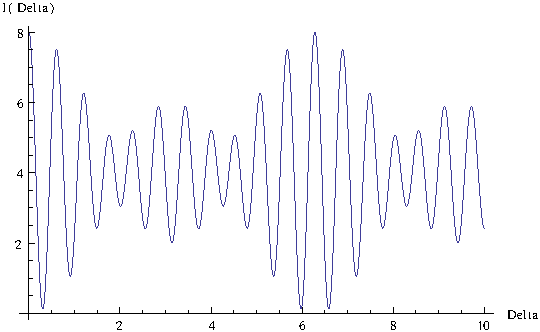
\includegraphics[width=0.5\textwidth]{schwebung.pdf}
	\caption{$I(t)$ für $f/a = 10$}
	\label{schwebung}
\end{figure}

Für Minimal- und Maximalwert ist die Einhüllende interessant. Aus einem Plot
mit $f/a = 100$, bei dem die einhüllende abzulesen ist, erhalte ich an den
extremsten Stellen $I_\text{max} = 8$ und $I_\text{min} = 0$. An den mittleren
Stellen ist $I_\text{max} = 6$ und $I_\text{min} = 2$. An den kontrastärmsten
Stellen ist $I_\text{max} = 5$ und $I_\text{min} = 3$. Somit sind die
Kontraste:
\[
	K = 1
	,\quad
	K' = \frac 12
	,\quad
	K'' = \frac 14
\]

%%%%%%%%%%%%%%%%%%%%%%%%%%%%%%%%%%%%%%%%%%%%%%%%%%%%%%%%%%%%%%%%%%%%%%%%%%%%%%%
%                Auflösungsvermögen abbildender Instrumente                 %
%%%%%%%%%%%%%%%%%%%%%%%%%%%%%%%%%%%%%%%%%%%%%%%%%%%%%%%%%%%%%%%%%%%%%%%%%%%%%%%

\section{Auflösungsvermögen abbildender Instrumente}
\label 2

\subsection{Digitalkameras}

Die numerische Apertur $N$ ist ungefähr:
\[
	N \approx \sin \phi \approx \frac rf = \frac D{2f}
\]

Angenommen, es handelt sich um eine Fotokamera mit quadratischen Pixeln (und
keine PAL oder HDV Videokamera), dann ist der Abstand $d$ zweier Pixel:
\[
	\frac{\unit{5}{\milli\meter}}{d} = \sqrt{8 \e 6}
	\iff
	d = \unit{1.77}{\micro\meter}
\]

Der Pixelabstand steht mit der numerischen Apertur in Verbindung:
\[
	d \approx \frac{\lambda}{N}
\]

Bei grünen Licht von $\lambda \approx \unit{500}{\nano\meter}$ müsste die
numerische Apertur der Optik mindestens $0.28$ sein, damit der Sensor an seine
Grenze kommt. Bei $f/D = 3.5$ ist die numerische Apertur allerdings $0.57$, so
dass das Objektiv der begrenzende Faktor ist. Das Objektiv würde erst bei einem
Pixelabstand von $\unit{875}{\nano\meter}$ an seine Grenzen kommen.

\begin{small}
	Für die Zielgruppe der Elektronikmarktwerbung ist wahrscheinlich die Angabe
	der Megapixel nicht das wichtigste. Ähnlich wie der Kilopreis beim
	Waschmittel ist die \emph{Megapixel pro Preis} Angabe viel wichtiger. So
	kommen einfache Spiegelreflexkameras auf $\unit{11}{\kilo \per \euro}$, die
	teuren Kameras jedoch nur auf $\unit{5}{\kilo \per \euro}$. Mobiltelefone
	liegen in dieser Hinsicht mit bis zu $\unit{30}{\kilo \per \euro}$ noch am
	besten.
\end{small}

\subsection{Mondlandung}

Die Brennweite des Spiegels ist:
\[
	f = \frac r2 = \unit{14.5}{\meter}
\]

Die Winkelauflösung des Systems ist: \cite[11.1.5]{meschede-gerthsen_24}
\[
	\phi \approx 1.22 \frac \lambda r = \unit{37}{\nano\radian}
\]

Bei einer Entfernung zum Mond von $\unit{380}{\mega\meter}$ entspricht dies
einem Abstand von $\unit{14}{\meter}$ auf dem Mond. Da die Raumfähre und der
Rover eher in der Größenordnung \unit{5}{\meter} sind, kann man sie daher mit
diesem Teleskop nicht sehen.

\begin{small}
	Unabhängig davon würden Skeptiker sich nicht mit einem Foto des Mondes
	zufrieden geben, weil man die Mondlandung dort sicher nachträglich
	eingearbeitet hätte.
\end{small}

%%%%%%%%%%%%%%%%%%%%%%%%%%%%%%%%%%%%%%%%%%%%%%%%%%%%%%%%%%%%%%%%%%%%%%%%%%%%%%%
%                Intensitätstransmission durch Polarisatoren                 %
%%%%%%%%%%%%%%%%%%%%%%%%%%%%%%%%%%%%%%%%%%%%%%%%%%%%%%%%%%%%%%%%%%%%%%%%%%%%%%%

\section{Intensitätstransmission durch Polarisatoren}
\label 3

\subsection{Polarisationsrichtung}

Nachdem das Licht durch den Linearpolarisator getreten ist, ist es linear
polarisiert.

\begin{figure}[H]
	\centering
	%\includegraphics[width=0.3\textwidth]{youdontsay.png}
	%\caption{Bild aus \cite{youdontsay}}
\end{figure}

Das zirkulär polarisierte Licht kann ich als Überlagerung von zwei ebenen
Wellen auffassen. Dabei sei die eine Welle in Richtung des Polarisators, die
andere senkrecht dazu. Beide Wellen haben die Amplitude $A_0$. Die Intensität
der Welle vor dem Polarisator ist dann:
\[
	A = \sqrt{A_0^2 + A_0^2} = \sqrt{2} A_0
\]

Die Intensität ist $I = A^2 = 2 A_0$. Nach dem Polarisator ist nur noch die
eine Welle da. Somit ist die Intensität nur noch $A_0^2 = I / 2$.

Bild stammt aus \cite{youdontsay}.

\subsection{}

Die Amplitude der nun linear polarisierten Welle wird durch einen Polarisator,
der um $\Theta$ verdreht ist, wird mit dem Faktor $\cos\del\Theta$
multipliziert.

Durch den letzten Polarisator wird das Licht dann noch um $\cos\del{\frac \pi 2
- \Theta}$ reduziert.

Die Intensität ist dann das Quadrat der Amplituden, also:
\[
	I_0 \cos^2\del\Theta \cos^2\del{\frac \pi 2 - \Theta}
\]

Wenn man den zweiten Polarisator weglässt, stehen die beiden verbleibenden
Polarisatoren senkrecht zueinander und somit kann kein Licht durchkommen, $I =
0$. Dies ist auch zu sehen, wenn man in die obige Formel $\Theta = 0$ oder
$\Theta = \pi/2$ einsetzt. Dann wird einer der Kosinusterme $0$.

\subsection{}

Ähnlich zur vorherigen Aufgabe ist der Faktor der Intensität:
\[
	\prod_{i = 1}^{n} \cos^2\del{\frac{\pi}{2(n-1)}}
\]

Im Grenzwert $n \to \infty$ wird das Argument des Kosinus klein, so dass ich es
um $0$ entwickeln kann. Alle Terme der Ordnung $\mathcal O\del{\frac{1}{n^2}}$
können vernachlässigt werden. Da $\cos(x) = 1 + \mathcal O\del{x^2}$, gilt
somit:
\[
	\lim_{n \to \infty} \prod_{i = 1}^{n} \cos^2\del{\frac{\pi}{2(n-1)}} = 1
\]

Unendlich viele ideale Polfilter können das Licht also ohne Intensitätsverlust
drehen.

\bibliography{../../zentrale_BibTeX/Central}
\bibliographystyle{plain}

\end{document}

% vim: spell spelllang=de
